\documentclass[mcp]{article}
%\documentclass[11pt, twocolumn]{article}

\usepackage[colorinlistoftodos]{todonotes}
\usepackage{graphicx}
\graphicspath{ {./images/} }

\usepackage{fullpage}
\usepackage{amsfonts,amsthm}
\usepackage{amsmath}
%\numberwithin{figure}{section} % numbering in each subsection
\numberwithin{table}{section}
\usepackage{setspace}
\usepackage{url}
\usepackage{lscape} %% rotating table
\usepackage{rotating}
\usepackage{authblk}
\usepackage{subcaption}
\usepackage{hyperref}
\usepackage{xcolor} %\[table,dvipsnames]
%\usepackage{makecell}
%\usepackage{array}

% remove number of section in the title
\makeatletter
\def\@seccntformat#1{%
  \expandafter\ifx\csname c@#1\endcsname\c@section\else
  \csname the#1\endcsname\quad
  \fi}
\makeatother

\usepackage{caption}

%% to remove zero preceding section number.
\renewcommand\thesection{\arabic{section}}
\renewcommand\thesubsection{\thesection.\arabic{subsection}}

\usepackage{tabulary,multirow,multicol,rotating}
\usepackage[backend=biber,sorting=none]{biblatex}
\addbibresource{bibliography.bib}

\definecolor{Red}{rgb}{0.60,0.00,0.00}
\definecolor{Blue}{rgb}{0.00,0.00,0.75}
\definecolor{LightYellow}{rgb}{1.00,0.97,0.68}
\definecolor{Green}{rgb}{0.30, 0.60, 0.30}
\definecolor{MyLightMagenta}{cmyk}{0.1,0.8,0,0.1} 
\definecolor{cornflowerblue}{rgb}{0.39, 0.58, 0.92}
\definecolor{darkorange}{rgb}{0.8, 0.4, 0}
\definecolor{LightPurple}{rgb}{1, 0.51, 0.98}
\definecolor{DarkPurple}{rgb}{0.54, 0.27, 0.53}
\definecolor{Purple1}{rgb}{0.83, 0.29, 0.95}
\definecolor{Purple2}{rgb}{0.97, 0.12, 0.59}
\definecolor{change}{rgb}{0.39, 0.58, 0.92}

\definecolor{function}{RGB}{0, 112, 192}
\definecolor{group}{rgb}{0.39, 0.58, 0.92}
\definecolor{ratio}{rgb}{1, 0.6, 0.16}
\definecolor{feature}{rgb}{0.83, 0.32, 0.48}
\definecolor{subject}{rgb}{0.6, 0.3, 0.09}
\definecolor{run}{rgb}{0, 0.68, 0.17}

\usepackage{array}
\newcolumntype{C}[1]{>{\centering\let\newline\\\arraybackslash\hspace{0pt}}m{#1}}
\setlength{\tabcolsep}{2pt}

%% for comments
\newcommand{\ignore}[1]{}
\def\todo#1{{\color{red}[#1]}}
\def\change#1{{\color{cornflowerblue}#1}}
\newenvironment{todolong}{\color{red}[TODO:}{]}
\def\note#1{{\color{OliveGreen}[NOTE: #1]}}
\def\added#1{{\color{blue}[ADDED: #1]}}
\def\devon#1{{\color{green}[4Devon: #1]}}

\def\eqref#1{Eq.~(\ref{eq:#1})}
\def\figshortref#1{{\bf Fig.~\ref{fig:#1}}}
\def\figref#1{{\bf Figure~\ref{fig:#1}}}
\def\secref#1{{\bf Section~\ref{sec:#1}}}
\def\tabref#1{{\bf Table~\ref{tab:#1}}}

\usepackage{xr}
\externaldocument[supp-]{../supplementary/ptm_sm}
%\def\sfigref#1{{\bf Supplementary Fig.~\ref{fig:#1}}}
%\def\snoteref#1{{\bf Supplementary Note~\ref{sec:#1}}}
%\def\snoteshortref#1{{\bf Suppl. Note~\ref{sec:#1}}}
%\def\stabref#1{{\bf Supplementary Table~\ref{tab:#1}}}

%%% should be change =2
\linespread{1}

%\date{\vspace{-5ex}} % to remove date in the title

\renewcommand{\deg}{\ensuremath{^{\circ}}\xspace}
\newcommand{\dd}[1]{\mathrm{d}#1}

%%%%%%%%%%%%%%%%%%%%%%%%%%%%%%%%%%%%%%%%%%%%%%%%%%%%%%%%%%%%%%%%%%%%%%%
%%%%%%%%%%%%%%%%%%%%%%%%%%%%%%%%%%%%%%%%%%%%%%%%%%%%%%%%%%%%%%%%%%%%%%%
%%%%%%%%%%%%%%%%%%%%%%%%%%%%%%%%%%%%%%%%%%%%%%%%%%%%%%%%%%%%%%%%%%%%%%%

\title{MSstatsPTM statistical relative quantification of post-translational modifications in bottom-up proteomic experiments}

\author[1]{Devon~Kohler}
\author[2]{Tsung-Heng~Tsai}
\author[1]{Ting~Huang}
\author[4]{Erik~Verschueren}
\author[3]{Trent~Hinkle}
\author[3]{Meena~Choi*}
\author[1]{Olga~Vitek*}
\affil[1]{Khoury College of Computer Science, Northeastern University, Boston, MA, USA}
\affil[2]{Kent State University, Kent, OH, USA}
\affil[3]{MPL, Genentech, South San Francisco, CA, USA}
\affil[4]{ULUA BV, Arendstraat 29, 2018 Antwerp, Belgium}
\affil[*]{Corresponding Authors}

\date{}

\begin{document}

\maketitle


%%%%%%%%%%%%%%%%%%%%%%%%%%%%%%%%%%%%%%%%%%%%%%%%%%%%%%%%%%%%%%%%%%%%%%%
%%%%%%%%%%%%%%%%%%%%%%%%%%%%%%%%%%%%%%%%%%%%%%%%%%%%%%%%%%%%%%%%%%%%%%%
\begin{abstract}

Mass spectrometry (MS)-based proteomics is increasingly used to detect changes in post-translational modifications (PTMs) between samples from various conditions. Analysis of data from such experiments faces numerous statistical challenges. These include the low abundance of modified proteoforms, the small number of representative peptides that span modification sites, and confounding between changes in the abundance of PTM and the overall changes in the protein abundance. Therefore, statistical approaches for detecting differential PTM abundance must integrate all the available information pertaining to a PTM site, and consider all the relevant sources of confounding and variation. In this manuscript we propose such a statistical framework, which is comprehensive, accurate, and leads to reproducible results. The framework requires an experimental design, which for each sample quantifies both the peptides with post-translational modifications, and peptides from the same proteins with no modification sites. The framework supports both label-free and tandem mass tag (TMT)-based acquisitions. The statistical methodology separately summarizes the abundances of peptides with and without the modification sites, and fits separate linear mixed effects models that reflect the biological and technological aspects of the experimental design. Next, model-based inferences regarding the PTM and the protein-level abundances are combined to account for the confounding between these two sources. Evaluations on computer simulations, a spike-in experiment with known ground truth, and three biological experiments demonstrate the improved fold change estimation and detection of differential PTM abundance, as compared to currently used approaches. The proposed framework is implemented in the free and open-source R/Bioconductor package $MSstatsPTM$. 

\end{abstract}

%%%%%%%%%%%%%%%%%%%%%%%%%%%%%%%%%%%%%%%%%%%%%%%%%%%%%%%%%%%%%%%%%%%%%%%
%%%%%%%%%%%%%%%%%%%%%%%%%%%%%%%%%%%%%%%%%%%%%%%%%%%%%%%%%%%%%%%%%%%%%%%
\clearpage
\section{Introduction}

\todo{This section would benefit from more biology/technology background, and more extensive references}
Signaling mechanisms allow cells to mount a fast and dynamic response to a multitude of bimolecular events. Signaling is facilitated by the modification of proteins at specific residues, acting as molecular on/off switches~\cite{Deribe,Cohen}. Localizing the modification sites, or characterizing relative abundance of a modification site's occupancy repertoire across experimental conditions, provides important insights~\cite{Mann}. For example, meaningful patterns of changes in post-translational modifications (PTMs) abundance can serve as biomarkers of a disease~\cite{Petushkova_2017}. Alternatively, distinguishing the quantitative changes in a PTM from the overall changes of the protein abundance helps gain insight into biological and physiological processes operating on a very short timescale \todo{would be good to have a reference}.

Bottom-up liquid chromatography coupled with tandem mass spectrometry (LC-MS/MS) is a tool-of-choice for unbiased and large-scale identification and quantification of proteins and their PTMs~\cite{Kall:2011ub,Roepstorff}. However, LC-MS-based interrogation of the modified proteome is challenging, for a number of reasons. First, the relatively lower abundance of modified proteoforms dictates that a global interrogation can only be achieved through large-scale enrichment protocols with modification-specific antibodies or beads \cite{Huang:2014}. Variability in the enrichment efficiency inevitably affects the reproducibility of the number of spectral features (e.g., peptide precursor ions or their fragments) and their intensities. Second, contrary to the often large number of identified peptides that can be used as features to model protein abundance changes, there are relatively few representative peptides that span a modification sites, which often results in sparse, and sometimes, inherently convoluted models (i.e., single versus multiple modified sites on a single peptide) \cite{Mann}. Third, unless early signaling events are interrogated, the interpretation of the relative changes in modification occupancy are inherently confounded with changes in the overall protein abundance, complication the interpretation of the results \cite{Olsen:2013}. Finally, technological aspects of bottom-up MS experiments, and presence of labeling, e.g. by tandem mass tag (TMT), introduce additional sources of uncertainty and variation.

The technological challenges in PTM identification and quantification translate themselves into challenges of statistical data analyses. Yet frequently data from these experiments are analyzed using statistical methods that were not originally designed for this task. In particular, methods such as t-test, Analysis of Variance, or Limma take as input the intensity ratios of modified and unmodified peptide features, and compare the mean abundance of different PTM sites~ \cite{Ritchie_15a}. Such methods do not fully account for all the sources of uncertainty and variation in the experiment. As the result, they are either not directly applicable to experiments with non-trivial designs (such as experiments with multiple conditions, paired and time course designs, and experiments with labeling), or require the analysts to exercise non-trivial statistical expertise.

This manuscript proposes a general statistical analysis framework that detects relative changes in post-translational modifications. The framework requires an experimental design, which for each sample quantifies both the peptides with post-translational modifications, and peptides from the same proteins with no modification sites. The framework supports both label-free (DIA, DDA) and tandem mass tag (DDA-TMT)-based acquisitions. The statistical methodology separately summarizes the abundances of peptides with and without the modification sites, and fits separate linear mixed effects models that reflect the biological and technological aspects of the experimental design. Next, model-based inferences regarding the PTM and the protein-level abundances are combined to account for the confounding between these two sources.

We evaluated the proposed framework on \todo{how many} datasets from computer simulations, \todo{how many} benchmark controlled mixtures, and \todo{how many} biological investigations. The datasets illustrate a diverse set of organisms, acquisition methods, and experimental designs, showing the applicability of the framework to a variety of situations. The evaluations demonstrated that by appropriately leveraging the information from the unmodified peptide, the proposed approach improves the accuracy of the estimates of PTM fold changes and results in a better calibrated false positive rate of detecting differentially abundant PTMs. In particular, accounting for the confounding from protein abundance allows us to characterize the true effect of the modification, avoiding the need for more manual and time intensive methods.

The proposed approach is implemented as a freely available open source R package $MSstatsPTM$, available on Bioconductor, which employs similar input format as in $MSstats$ and $MSstatsTMT$ \cite{Choi:2014,Huang:2020}.

\section{Experimental Procedures}

The benchmark datasets in this manuscript provide a performance benchmark of the proposed approach in situations with known ground truth, and to represent a variety of experimental designs and acquisition methods. Two computer simulations varied in experimental realism. The first simulation produced a perfectly clean dataset, with many replicates and no missing values. The second simulation introduced real-world characteristics, such as limited modified features and missing values. The spike-in experiment took the real world characteristics a step further and allowed us to compare the methods in a real experiment with known changes in modified spike-in peptides. Finally, three biological experiments demonstrated the applicability of the proposed approach across different biological organisms, experimental designs, and data acquisition strategies. Table \ref{tab:dataDescription} summarizes the experiments. Details of the experimental data, R scripts with $MSstatsPTM$ analysis, and the results of the statistical analysis are available in either MassIVE.quant \todo{cite the paper, provide url}. Details of computer simulations are available on GitHub.

%%%% Summary of controlled mixtures
\begin{table}[h!]
\centering
\begin{tiny}
\begin{tabular}{|c|c|ccc|c|}
\hline
%%%% colnames of table
& \multirow{2}{*}{Dataset} & Experimental & No. of & No. of Bio. &  Data \\
&  & Design & Conditions & Replicates & availability \\
\hline
\hline
 &&&&& \\[-0.05in]
%%%% DDA:ControlledMix
\multirow{5}{*}{\rotatebox[origin=c]{90}{Known}}  \multirow{5}{*}{\rotatebox[origin=c]{90}{Ground}} \multirow{5}{*}{\rotatebox[origin=c]{90}{Truth}} & Computer simulation 1 - Label-free & Group comparison & 2/3/4 & 2/3/5/10 & \href{https://github.com/devonjkohler/MSstatsPTM_simulations}{Github \todo{url?}}\\
 &&&&& \\%[-0.05in]
%\hline 
%&&&&&&&& \\[-0.05in]
% \cline{2-9}
% &&&&&&&& \\[-0.05in]
%%% DDA iPRG2015
& Computer simulation 2 - missing and low features & Group comparison & 2/3/4 & 2/3/5/10 & \href{https://github.com/devonjkohler/MSstatsPTM_simulations}{Github \todo{url?}} \\
 &&&&& \\%[0.05in]
%\hline 
% &&&&&& \\[-0.05in]
%%% DDA Cox2014
& SpikeIn benchmark - Ubiquitination - Label-free & Group comparison & 4 & 2 & \href{https://massive.ucsd.edu/ProteoSAFe/private-dataset.jsp?task=c4c583ecf7f941cdac87f7a4f872517b}{MSV000088971}\\
 &&&&& \\%[-0.05in]
\hline
\multicolumn{6}{c}{ } \\ [0.02in]
\hline 
 &&&&& \\%[-0.05in]
%%%%%%%%%%%%%%%%%%
%%%% biological study
%%%%%%%%%%%%%%%%%%
%% DDA Meierhofer
\multirow{3}{*}{\rotatebox[origin=c]{90}{Biological}} \multirow{3}{*}{\rotatebox[origin=c]{90}{Investigation}} & Human - Ubiquitination - 1mix-TMT & Group comparison & 6 & 2 & \href{https://massive.ucsd.edu/ProteoSAFe/dataset.jsp?task=b6f0c74c234247678fb0888c6df1f225}{MSV000088966} \\
&&&&& \\%[-0.05in]
% \cline{2-9}
% &&&&&&& \\[-0.05in]
%%%% SRM Picotti 2009
& Mouse - Phosphorylation - 2mix-TMT & Time course & 6 & 4 & \href{https://massive.ucsd.edu/ProteoSAFe/dataset.jsp?task=4878d777c6b34cf8aaf8477e93140c4d}{MSV000085565} \\
&&&&& \\%[-0.05in]
% \cline{2-9}
% &&&&&&& \\[-0.05in]
%%%% SRM Surinova 2015, training
& Human - Ubiquitination - Label-free & Group comparison & 4 & 2 & \href{https://massive.ucsd.edu/ProteoSAFe/dataset.jsp?task=1b516164de5345108b40b75147dd58b5}{MSV000078977}\\ [0.02in]
 &&&&& \\
 \hline
\end{tabular}\\
\end{tiny}
\caption{ \small {\bf Simulated and experimental datasets in this manuscript} 
```Dataset'' is the code name of the dataset in this manuscript.
``Data availability'' shows the ID of the MassIVE.quant repository \todo{url} or the GitHub repository. 
}
\label{tab:dataDescription}
\end{table}

\subsection*{Dataset 1 : Computer simulation 1 - Label-free}
\label{sec:comp_sim_procedure1}

The simulation mimicked a label-free experiment. Synthetic datasets had a high number of modified peptide features and no missing values, while varying numbers of replicates and conditions. Specifically, each dataset had 1000 PTMs and 1000 unmodified proteins, each represented by 10 LC-MS features observed across all the mass spectrometry runs. 500 of the PTMs were generated with a differential fold change between conditions, while the other half were generated with no difference between conditions. Of the 500 differential PTMs, the fold change of 250 were fully masked by changes in the unmodified protein. Of the 500 non-differential PTMs, 250 were generated with a differential fold change that was entirely due to the unmodified protein. All differential PTMs were generated with an expected log fold change of .75 between conditions. Each simulation was generated with random biological variation. Specifically, let $Y_{ibc}$ denote the abundance of peptide $i$ in biological replicate $b$ of condition $c$. The simulated peptide abundance  $Z_{ibc}$ was generated as $Z_{ibc} = Y_{ibc} + \epsilon_{ibc}$ where $\epsilon_{ibc}\sim^{iid}N(0,\sigma^2)$. The simulations were generated with one of two values $\sigma^2 = \{.2, .3\}$ motivated by the biological experiments in this manuscript.

Further details of how the first simulation was generated, can be found in Supplementary Sec. \ref{supp-sec:dataset1}.

\subsection*{Dataset 2 : Computer simulation 2 - Label-free missing values and low features}
\label{sec:comp_sim_procedure2}

In this simulation, data was generated using the same parameters as described in the previous section and including real world experimental conditions. Specifically these simulations included missing values and a low number of modified features. The percentage of missing values and feature counts were determined by looking at the biological experiments in this paper. PTMs were simulated with 2 modified peptide features, while unmodified proteins were still simulated with 10 features. Additionally, 20\% of observations for both modified and unmodified peptides were missing completely at random. Adding missing values and few representative modified features provides a more realistic expectation of model performance.

Further details of how this simulation was generated, including exact parameters used, can be found in Supplementary Sec. \ref{supp-sec:dataset2}.
 
\subsection*{Dataset 3 : SpikeIn benchmark - Ubiquitination - Label-free}
\label{sec:exp_proc_dataset3}
We evaluated our approach using a custom designed spike-in benchmark experiment with known ground truth. This experiment had 4 conditions with two biological replicates per condition and a balanced design.

Experimental Design: In this experiment 50 heavy-labeled KGG motif peptides from 20 human proteins were used as spike-in peptides. Quantitative changes in protein and site abundance of these 20 proteins were the target of the benchmark.  Unmodified peptides from Human Lysate were used as the estimate of global protein abundance changes. Background E coli Lysate was used to normalize total protein levels prior to enrichment or global protein profiling. The background lysate was treated as controls and are not expected to be differential in any comparison. The spike-in peptides were mixed with human lysate to create four mixture conditions. Two sets of data were acquired for each mixture: KGG enriched + LC-MS, and LC-MS only.

Global Profiling Run: This experiment included a separate global profiling run to measure unmodified peptides. There was a 90.2\% overlap between the identified background modified peptides and proteins that were quantified in the global profiling run.

Pairwise Comparisons: We evaluated the ability of the methods to detect known changes in abundance between pairs of conditions. The four mixtures were treated as individual conditions and labeled mix1, mix2, mix3, and mix4. The pairwise comparisons were mix1-mix2, mix1-mix3, mix1-mix4, mix2-mix3, mix2-mix4, and mix3-mix4. The true log fold changes of spike-in modified peptides in these comparisons can be seen in Table \ref{table:spikein_fold_change}.

\begin{table}[h!]
\centering
\begin{tabular}{| c | c |}
\hline
 Comparison & Expected log fold change\\ [0.5ex]
 \hline\hline
 mix1-mix2 & -1\\
 \hline
 mix1-mix3 & 1\\
\hline
 mix1-mix4 & 0\\
\hline
 mix2-mix3 & -2\\
\hline
 mix2-mix4 & -1\\
\hline
 mix3-mix4 & 1\\
\hline
\end{tabular}
\caption{The expected log fold change of modified spike-in peptides in Dataset 3.}
\label{table:spikein_fold_change}
\end{table}

More information on the experimental design of the benchmark experiment and how the expected fold change was calculated can be found in Supplementary Sec. \ref{supp-sec:benchmark}.

\subsection*{Dataset 4 : Human - Ubiquitination - 1mix-TMT}
\label{sec:exp_proc_dataset4}
The proposed approach was evaluated on an experiment with six conditions and an unbalanced design.

Experimental Design: In this study Luchetti et al. \cite{LUCHETTI2021} used multiplex proteomics to quantify the abundance of total protein and ubiquitination in human epithelial cells. Cells were engineered to express IpaH7.8 under a dox inducible promoter and measurements were taken at different time periods. GSDMD was actively degraded when IpaH7.8 expression was induced by dox treatment. Uninfected cells were measured at 0 and 6 hours, while infected cells were measured at 1, 2, 4, and 6 hour increments, resulting in six total conditions.

Global Profiling Run: This experiment included a separate global profiling run to measure unmodified peptides. There was a 95\% overlap between the identified modified peptides and proteins that were quantified in the global profiling run.

Pairwise comparisons: We evaluated the statistical approach by its ability to detect changes in the abundance of modified peptides both before and after adjusting for changes in global protein abundance. The six condition were labeled Dox1hr, Dox2hr, Dox4hr, Dox6hr, NoDox0hr, and NoDox6hr. All conditions were compared with each other in a full pairwise comparison, resulting in 15 comparisons. Because the dataset is a biological investigation, the true positive modifications were unknown.

Further details on the design of this experiment are provided in Supplementary Sec. \ref{supp-sec:ipah}. 

\subsection*{Dataset 5 : Mouse - Phosphorylation - 2mix-TMT time series}
\label{sec:exp_proc_dataset5}
In this experiment 8 biological replicates were allocated to 2 TMT mixtures in an unbalanced design.

Experimental Design: Maculins et al. \cite{Maculins} designed an experiment targeting primary murine macrophages infected with Shigella flexneri (S.flexneri). Multiplex proteomics was used to quantify the abundance of total protein, and phosphorylation in wild type (WT) and ATG16L1-deficient (cKO) samples, uninfected and uninfected with S.flexneri. The abundance of total protein and post-translation modifications were quantified at three time points, uninfected, early infection (45-60 minutes), and late infection (3-3.5 hours). 11-plex isobaric multiplexing via tandem mass tagging (TMT) in combination with liquid-chromatography and tandem mass spectrometry (LC-MS/MS) was used. Six conditions were split between 11 channels leading to the experimental design being unbalanced. Each mixture contained two replicates per early and late WT and KO conditions. Mixture one contained one replicate of uninfected WT and two replicates of uninfected KO. Mixture two contained one replicate of uninfected KO and two uninfected WT.

Global Profiling Run: This experiment included a separate global profiling run to measure unmodified peptides. There was a 90\% overlap between the identified background modified peptides and proteins that were quantified in the global profiling run.

Time series comparison: We evaluated the statistical approach by its ability to detect changes in the abundance of modified peptides both before and after adjusting for changes in global protein abundance. The six condition were labeled KO\_Uninfect, KO\_Early, KO\_Late, WT\_Uninfect, WT\_Early, and WT\_Late. 9 total comparisons were made named KO\_Early-WT\_Early, KO\_Late-WT\_Late, KO\_Uninfected-WT\_Uninfected, KO\_Early-KO\_Uninfected, KO\_Late-KO\_Uninfected, WT\_Early-WT\_Uninfected, WT\_Late-WT\_Uninfected, Infected-Uninfected, and KO-WT. Because the dataset is a biological investigation, the true positive modifications were unknown.

Further details on the design of this experiment are provided in Supplementary Sec. \ref{supp-sec:shigella}.

\subsection*{Dataset 6 : Human - Ubiquitination - Label-free no global profiling run}
\label{sec:exp_proc_dataset6}

In this experiment 8 biological replicates were split between 4 conditions in a balanced design.

Experimental Design: Cunningham et al. \cite{Cunningham2015} investigated the relationship between USP30 and protein kinase PINK1, and their association with Parkinson’s Disease. Ubiquitination site profiling was performed and the modified site abundance was analyzed. Four conditions were tested with two biological replicates per condition. The conditions were as follows: CCCP, USP30 over expression (USP30 OE), Combo, and Control. Label-free mass spectrometry quantification was used to quantify the abundance of modified peptides.

Global Profiling Run: This experiment did not included a separate global profiling run to measure unmodified peptides. In this case $MSstatsPTM$ can still be used by extracting unmodified peptides from the modified run, however this leads to substantially less matches between modified and unmodified peptides, in addition to low feature counts for unmodified peptides. There was a 41.9\% overlap between the identified background modified peptides and proteins that were quantified in the global profiling run.

Pairwise comparisons: We evaluated the statistical approach by its ability to detect changes in the abundance of modified peptides both before and after adjusting for changes in global protein abundance. The four condition were labeled CCCP, Combo, Ctrl, and USP30\_OE. All conditions were compared with each other in a full pairwise comparison, resulting in 6 comparisons. Because the dataset is a biological investigation, the true positive modifications were unknown.

%%%%%%%%%%%%%%%%%%%%%%%%%%%%%%%%%%%%%%%%%%%%%%%%%%%%%%%%%%%%%%%%%%%%%%%
\section*{Results}

\subsection*{Existing statistical methods for experiments targeting PTMs}

Despite the important implications of PTMs in biological functions, there is a lack of general framework to summarize the available quantitative information from LC-MS data, to perform statistical inference, and to draw conclusions to characterize the quantitative properties of PTM in a statistically rigorous manner. Many investigations performed differential abundance analysis of PTMs using two-sample t-test or its extensions. The approach takes as input intensities of individual features from modified peptides, or intensity ratios of modified and unmodified peptide features, and compares the mean abundance of a PTM site from one condition to another. Modifications of the t-test such as moderated t-test with Limma were also proposed \cite{Zhu}. While simple, the approach does not fully account for the sources of variations, and it is not directly applicable to experiments with complex designs, e.g., comparisons of multiple conditions, acquisition in multiple batches, etc. Additionally, while this approach can be applied to experiments targeting PTMs, there is not a self contained, straight forward implementation of the methods, making application challenging. 

Isobar-PTM was developed for experiments with MS/MS quantitative strategies that employ isobaric labels such as tandem mass tags (TMT) and isobaric tag for relative and absolute quantification (iTRAQ)\cite{Breitwieser:2013}. Isobar-PTM expresses MS measurements with a linear model and performs adjustment with respect to protein abundance using the difference between log-ratio of modified peptides in two channels and log-ratio of protein level. The modeling framework, however, is not applicable for either label-free workflows or experiments with complex designs. 

Further details on the specific equations and workflow of existing methods can be seen in Supplementary Sec. \ref{supp-sec:ttest}.

\subsection*{Proposed approach}

Figure \ref{fig:data-structure} schematically illustrates a simplified version of the data structure resulting from a typical bottom-up experiment for quantitative analysis of PTMs, in which there are multiple layers of variation present. A PTM site is quantified with multiple spectral features, which vary in sequence (e.g., fully or partially cleaved peptides), ionization efficiency, charge states, etc. The number quantified features vary across replicate LC-MS/MS runs of the same sample, and across conditions. To perform adjustment with respect to protein abundance, features of unmodified peptides are used for the inference of underlying protein abundance. Typically, because of the enrichment step for PTMs, very few of those features are present in original LC-MS runs. For more accurate estimation of protein abundance, separate global proteomics data of unenriched samples are recommended. If unmodified peptides are unavailable for any given modification, unmodified intensity adjustment cannot be performed. As different levels of variability are present in the data, the log-intensities of the features for modified and unmodified peptides are modeled separately using two linear mixed models.

%%%%%%%%%%%%%%%%%%%%%%%%%%%%%%%%%%%%%%%%%%%%%%%%%%%%%%%%%%%%%%%%%%%%%%%
\subsubsection*{Existing work in statistical modeling and parameter estimation}

The proposed approach leverages the large amount of work done to create $MSstats$~\cite{Choi:2014}. It takes as input a list of log-transformed intensities of spectral features, identified and quantified across LC-MS runs. The features, which are precursor ions of modified or unmodified peptides, are used to characterize the identified PTM sites and proteins. For each PTM site, the feature log-intensities of the modified peptides spanning the site are expressed using a linear mixed model in consideration of the effects of condition, run, feature and interaction between run and feature. The model parameters are estimated using the split-plot approach as in $MSstats$, where the feature log-intensities are first summarized into a single value per site per run in the subplot model, and the site-level summaries are then used for the inference of the PTM site abundance \cite{Choi:2014}. This approach allows the method to be extended to cases where the experimental design is unbalanced, and where additional sources of variation are present. In the site-level summarization, Tukey's median polish (TMP), a simple and robust procedure is applied to iteratively fit a two-way additive model with the effects of run and feature, which in turn summarizes the log-intensities for each site \cite{Tukey:1977}. After summarization, the inference of the PTM site abundance in each condition is carried through fitting a model based on the family of linear mixed-effects models \cite{Bolker2009} \cite{Faraway:2006}. Statistical modeling and quantification for global proteomics data are performed by the same procedure as for PTM data.

Additionally, the proposed method can include imputing missing feature intensities if desired. When values are imputed, it is assumed they are missing for reasons of low abundance. Missing features are imputed in each MS run using the Accelerated Time Failure (AFT) model \cite{Tukey:1977}. In order to impute a feature's missing values, the feature must be present in at least one MS Run. If the feature is not present across all MS Runs, the value will be left missing. Missing value imputation is done before summarization with Tukey's Median Polish in order to correct for the impact of outliers. Missing value imputation is done separately for both the PTM and global protein datasets.

%%%%%%%%%%%%%%%%%%%%%%%%%%%%%%%%%%%%%%%%%%%%%%%%%%%%%%%%%%%%%%%%%%%%%%%
\subsubsection*{Detection of changes in PTMs - Balanced design with one source of variation}
\label{sec:adjustment_summary}

Here we propose a statistical method for detecting changes in PTMs and removing confounding with changes in global protein abundance. The method is shown when applied to a balanced design with multiple conditions and one technical replicate. In practice the experimental design can be unbalanced and variation can come from multiple sources. We show how the methods can be applied to more complex experimental designs in the next section.

Detection of differentially modified PTM sites is performed through testing the null hypothesis of ‘no change’ against the alternative. The null hypothesis states that there is no difference in log-abundance of the PTM site between conditions, adjusted with respect to protein abundance. There are $I$ conditions and $J$ mass spectrometry runs (technical replicates) per condition in the experiment. The PTM site is represented by $K$ spectral features (peptide ions, distinguished by their cleavage residues and charge states). The log-intensity (base 2) of Feature $k$, in Run $j$ of Condition $i$ is denoted by $y_{ijk}^{\ast}$. Conversely, the log-intensity of Feature $l$ from the unmodified peptides in the same run is denoted by $y_{ijl}$. The expected values of log-abundances of the PTM and protein in Condition $i$ are denoted by $\mu_{i}^{\ast}$ and $\mu_{i}$. The feature and run level summarization for condition $i$ is denoted as $\hat{y}_{i+}^{\ast}$ for the modified peptide and $\hat{y}_{i+}$ for the unmodified peptide. For two conditions $i$ and $i'$ the hypothesis test is formulated as follows:

\begin{equation}
\begin{aligned}
H_{0}: \Delta = ( \mu_{i}^{\ast} - \mu_{i'}^{\ast} ) - ( \mu_{i} - \mu_{i'} ) = 0 \\
H_{a}: \Delta = ( \mu_{i}^{\ast} - \mu_{i'}^{\ast} ) - ( \mu_{i} - \mu_{i'} ) \neq 0
\end{aligned}
\label{eq_1}
\end{equation}

Specifically, the adjusted difference is given by the difference in log-abundance of the PTM site, subtracted by the difference in log-abundance of the underlying protein, which is equivalent to the log of the ratio of PTM abundance difference to protein abundance difference. 

\begin{equation}
\hat{\Delta} = \left[ \frac{1}{J} \left( \hat{y}_{i+}^{\ast} - \hat{y}_{i'+}^{\ast} \right) \right] - \left[ \frac{1}{J} \left( \hat{y}_{i+} - \hat{y}_{i'+} \right) \right]
\end{equation}

The estimate of the adjusted difference and the standard error (SE) of the estimate are obtained by combining the difference estimates and the associated SEs from both counterparts.

\begin{equation}
SE(\hat{\Delta}) = \left[ \left( \hat{\sigma}_{\gamma^{\ast}}^{2} + \hat{\sigma}_{\gamma}^{2} \right) \right]^{1/2}
\end{equation}

Finally the degrees of freedom are calculated using the following formula.

\begin{equation}
\left( \hat{\sigma}_{\gamma^{\ast}}^{2} + \hat{\sigma}_{\gamma}^{2} \right)^2 \bigg/
\left( \frac{\hat{\sigma}_{\gamma^{\ast}}^{4}}{\mathrm{df}(\gamma^{\ast})} + \frac{\hat{\sigma}_{\gamma}^{4}}{ \mathrm{df}(\gamma)} \right)
\end{equation}

The test statistic for the hypothesis testing is the ratio of the estimate of the adjusted difference to its SE. To determine the statistical significance of the difference in terms of p-value, the test statistic is compared against the t distribution with degrees of freedom approximated by the Satterthwaite method\cite{satterthwaite:1946}. Adjustment for multiple comparisons is performed using the Benjamini-Hochberg procedure to control the false discovery rate at a desired level, e.g., $0.05$\cite{Benjamini:1995}.

\subsubsection*{Design of PTM experiments in the balanced case}
\label{sec:design}

The proposed statistical framework allows for design of PTM experiments in terms of sample size calculation and power analysis. 
%Sample size calculation based on linear models has been described for general applications~\cite{kutner_etal_04a} and specifically for protein significance analysis~\cite{oberg_vitek_09a}. 
Sample size calculation takes as input a) $q$, the desired false discovery rate, b) $\beta$, the average Type II error rate, c) $\Delta$, the minimal log-fold change in adjusted PTM abundance that we would like to detect, d) $m_0 / (m_0 + m_1)$, the fraction of truly differentially modified PTM sites in the comparison, and e) $\sigma_{\gamma^{\ast}}^{2}$ and $\sigma_{\gamma}^{2}$, the anticipated variances associated to modified and unmodified peptide features, respectively. The variances can be derived based on the dataset being analyzed, assuming similar quantitative properties and variations. With these values and a user-specified number of conditions, the corresponding number of technical replicates per condition can then be derived, as described in~\cite{kutner_etal_04a}. Given the above quantities, the minimal number of replicates $J$ is determined by the variance of the estimated log-fold change $\mathrm{SE}^{2}(\hat{\Delta})$ as

\begin{equation}
\mathrm{SE}^{2}(\hat{\Delta}) = \left[ \frac{2}{J} \left( \hat{\sigma}_{\gamma^{\ast}}^{2} + \hat{\sigma}_{\gamma}^{2} \right) \right]
\leq \left( \frac{\Delta}{t_{1-\beta, df} + t_{1-\alpha /2, df}} \right)^{2}
\end{equation}
where 
\begin{equation}
\alpha = (1 - \beta) \cdot \frac{q}{1 + (1-q) \cdot m_0 / m_1}
\end{equation}

and $t_{1-\beta, df}$ and $t_{1-\alpha /2, df}$ are the $100(1-\beta)^{\text{th}}$ and the $100(1-\alpha /2)^{\text{th}}$ percentiles of the $t$ distribution, with $df = I(J-1)$ degrees of freedom in balanced designs. 

Solving for J, the number of biological replicates per group is calculated as 

\begin{equation}
J \geq \frac{(2\hat{\sigma}_{\gamma^{\ast}}^{2} + 2\hat{\sigma}_{\gamma}^{2})(t_{1-\beta, df} + t_{1-\alpha /2, df})^2}{\Delta^2}
\end{equation}

More details on sample size calculation can be found in~\cite{oberg_vitek_09a}. 

%%%%%%%%%%%%%%%%%%%%%%%%%%%%%%%%%%%%%%%%%%%%%%%%%%%%%%%%%%%%%%%%%%%%%%%
%\subsection*{Analysis with multiple batches}

%The proposed statistical framework allows to analyze data from experiments of complex designs such as factorial design. We discuss below a specific design commonly considered in PTM experiments, in which data are acquired in multiple batches, often as a result of multiple repeats for the antibody enrichment step. Typically, the number of spectral features and their intensities are different across batches, and the run-to-run variation sometimes varies across batches as well. The proposed approach summarizes log-intensities in each batch separately, and considers two ways to perform the statistical inference and testing. When variability in site-level summaries and in PTM changes is expected across batches, the proposed approach performs inference of the PTM site abundance and the adjusted difference for each batch separately. The evidence about differential PTM sites between conditions is averaged over batches. Alternatively, assuming identical variability in the site-level summaries and identical differences between conditions across batches (i.e., no interaction effect between condition and batch), the statistical inference and testing can be performed based on one single model with an additional fixed effect of batch. Details about these modeling considerations are discussed in Supplementary Sec \ref{supp-sec:test}.

%%%%%%%%%%%%%%%%%%%%%%%%%%%%%%%%%%%%%%%%%%%%%%%%%%%%%%%%%%%%%%%%%%%%%%%
\subsubsection*{Detection of changes in PTMs - Extension to complex designs}

The statistical modeling approaches discussed above can also be extended to complex designs including experiments with additional sources of variation and unbalanced designs. Equation 1 is the same in this case and the null hypothesis is still that there is no difference in mean PTM abundance between Conditions $i$ and $i'$ after adjusting for changes in mean unmodified peptide abundance between Conditions $i$ and $i'$. 

Model inference is done in the same way to how MSstats~\cite{Choi:2014} and MSstatsTMT~\cite{Huang:2020} target the global protein. In cases where the design is unbalanced, a linear mixed effects model is fit, which takes into account all potential sources of variation, and restricted maximum likelihood (RML) is used to estimate the parameters of each model. Once the parameters are estimated, we can combine the models using modified versions of Equations 2, 3, and 4.

The log-fold change in the adjusted PTM abundance, $\Delta$, is now estimated by RML, and Equation 2 becomes 
\begin{equation}
\hat{\Delta} = (\hat{\mu}_{RML_i}^{\ast} - \hat{\mu}_{RML_{i'}}^{\ast}) - (\hat{\mu}_{RML_i} - \hat{\mu}_{RML_{i'}})
\end{equation}

The standard error of the estimate $\mathrm{SE}(\hat{\Delta})$ and degrees of freedom in Equations 3 and 4 are unchanged from the balanced case, although $\hat{\sigma}_{\gamma^z\ast}$ and $\hat{\sigma}_{\gamma}$ are now estimated using RML.

Details on how the proposed method can be used to run sample size calculations and power analysis on experiments with complex design can be seen in Supplementary Sec. \ref{supp-sec:complex_design}

\subsection*{Implementation}

The proposed methods are implemented in the open source R package $MSstatsPTM$, available on Bioconductor. $MSstatsPTM$ includes converters for multiple spectral processing tools, including MaxQuant, Progenesis, and Spectronaut. The converters take as input the raw data from the tool, identify the modification site for modified peptide, and put the data into the correct format for analysis in $MSstatsPTM$. Conversion is done separately for the modified and global profiling runs. If the global profiling run is not available, the package can still analyze the modified run, but will do so without adjusting for changes in unmodified protein abundance. Specifically, if a global profiling run is not available the null and alternative hypothesis in Equation \ref{eq_1} will reduce to:

\begin{equation}
\begin{aligned}
H_{0}: \Delta = \mu_{i}^{\ast} - \mu_{i} = 0 \\
H_{a}: \Delta = \mu_{i}^{\ast} - \mu_{i} \neq 0
\end{aligned}
\label{eq_9}
\end{equation}

Which amounts to running the methods seen in MSstats and MSstatsTMT on peptide level data \cite{Choi:2014} \cite{Huang:2020}.

After using the converters, the next step is peptide/protein summarization and missing value imputation. In the methods sections it was assumed that all the input data was summarized; in the implementation we need to run a specific summarization step to make this happen. For the modified run, the package summarizes features, PSMs, which include the same modification together. Features with multiple modification sites are not included with single site features and are summarized separately. For the global profiling run all unmodified features from the same protein are summarized together, up to the protein level. Additionally, the summarization includes global median normalization and normalizes between MS runs. The package uses an AFT model to impute missing values, although this step is optional.

The final step of the package is modeling the summarized dataset. A linear mixed effects model is fit for both the summarized modified and global profiling runs. This model is automatically adjusted depending on the experimental design and acquisition method. The comparisons of interest can either be predefined or a full pairwise comparison will be tested. After fitting a model to both the modified and unmodified data, the modified model is adjusted for changes in unmodified protein abundance, using the methods described in this paper. 

Beyond the core functionalities of conversion, summary, and modeling, the package also includes functions for plotting the results. These include plots for the summarized and modeled data to assist in the analysis of the experiment. The summarized plots help with quality assurance analysis and identifying sources of variation. This includes a quality control plot, summarizing the peptide abundance per run in the form of a boxplot, and a profile plot, plotting each feature and the overall feature summarization as a line plot over each run. Additionally, the model plots include a volcano plot, showing all peptides adjusted pvalues and fold changes, as well as a heatmap, which evaluates the fold change between conditions and peptides. 

The package relies on functionalities from the R packages $MSstats$ \cite{Choi:2014} and $MSstatsTMT$ \cite{Huang:2020}. The statistical modeling relies on the functionality from the R packages $lme4$ \cite{Bates2015} and $lmerTest$ \cite{Kuznetsova2017}. An overview of the steps of the package are illustrated in Figure \ref{fig:msstatsptm_design}.

The code is available on Bioconductor, \url{http://www.bioconductor.org/packages/release/bioc/html/MSstatsPTM.html}, and Github, \url{https://github.com/Vitek-Lab/MSstatsPTM}.

%%%%%%%%%%%%%%%%%%%%%%%%%%%%%%%%%%%%%%%%%%%%%%%%%%%%%%%%%%%%%%%%%%%%%%%
%%%%%%%%%%%%%%%%%%%%%%%%%%%%%%%%%%%%%%%%%%%%%%%%%%%%%%%%%%%%%%%%%%%%%%%
\subsection*{Evaluation}

The performance of the proposed method was evaluated on simulated and spike in datasets with known ground truth, as well as biological experimental data where the ground truth was not known. For the experiments where ground truth was known, we calculated the number of true positives (TP), false positives (FP), true negatives (TN), and false negatives (FN). True positives were modified peptides that are differential after accounting for changes in global protein abundance. True negatives were modified peptides that were not differentially abundant after accounting for global protein abundance. To determine positives and negatives we adjusted the p-values for multiple testing and used an $\alpha=.05$ cutoff to determine differential sites. These results were then compared to the ground truth to determine TP and TN. We used these results to calculate the false discovery rate (FDR = FP/(TP+FP)), the recall rate (TP/(TP + FN), and accuracy ((TP + TN) / (TP + TN + FP + FN)). Finally, the summary statistics were compared across methods to analyze method performance. 

For biological experiments where ground truth was not known, we adjusted the p-values for multiple testing and used an $\alpha=.05$ cutoff to determine differential sites. Comparisons were made before and after adjusting for changes in unmodified protein abundance and differences between the comparisons were noted. Each biological dataset presented a different experimental scenario, showing the applicability of the proposed method on a variety of experimental designs. All datasets in this paper were evaluated using the $MSstatsPTM$ package.

%%%%%%%%%%%%%%%%%%%%%%%%%%%%%%%%%%%%%%%%%%%%%%%%%%%%%%%%%%%%%%%%%%%%%%%
\subsubsection*{The proposed approach corrects for high FDR in computer simulations}

The proposed approach was evaluated against two-sample t-test and Limma in computer simulations. 
In Figure \ref{fig:sim1_fdr} we see that not accounting for changes in unmodified peptide level results in a high false discovery rate. When adjusting for changes in the unmodified peptide, all methods performed similarly in terms of FDR. In a clean simulation, recall and accuracy of the proposed approach and Limma performed similarly, with Limma performing slightly better with low replicates. In contrast, the performance of the t-test method lagged behind the others. Two-sample t-test only uses data within the groups of interest while ignoring the remainder of the data, leading to similar performance across all simulations. In contrast, the proposed approach and Limma leverage all available information, which resulted in improved power in simulations with more conditions.

%%%%%%%%%%%%%%%%%%%%%%%%%%%%%%%%%%%%%%%%%%%%%%%%%%%%%%%%%%%%%%%%%%%%%%%
\subsubsection*{The proposed approach outperforms existing methods in simulations with missing values and low features}

In this simulation the proposed method outperformed t-test and limma when real world experimental conditions were introduced. Changes in unmodified peptide level still needed to be accounted for to control the FDR. Once controlling for changes in the unmodified peptide, the proposed method out performed the other methods, as seen in Figure \ref{fig:sim2_acc}. The proposed method calibrated model accuracy and recall rate well, even when the number of replicates were low. Additionally, when comparing the fold change estimation across all peptides, the proposed method showed a tighter distribution of estimated fold changes around the true fold change than t-test and Limma. Specifically, the inner quartile range of the estimated fold change for the proposed method was on average 10.4\% smaller than t-test and 21.8\% smaller than Limma. This fold change comparison can be seen in Supplementary Figure \ref{supp-fig:fc_boxplot}.

Further details reviewing the results of each simulation and their comparison with respect to method performance can be seen in Supplementary Sec. \ref{supp-sec:sim}. 


%%%%%%%%%%%%%%%%%%%%%%%%%%%%%%%%%%%%%%%%%%%%%%%%%%%%%%%%%%%%%%%%%%%%%%%
\subsubsection*{In a label-free benchmark experiment the proposed approach corrects for bias and outperforms existing methods}

In this experiment all models incorrectly estimated the fold change of the modified spike-in peptides before adjusting for changes in global protein abundance. After adjustment, the spike-in peptides' fold change was in line with expectation (Figure \ref{fig:spikein_boxplot}). While the median fold change for the spike-in peptides was generally in line with the true fold change after adjustment, we can see that the distribution of fold changes for the peptides was visibly wider after adjustment. However, the proposed method a tighter distribution around the true log fold change. Comparing the inner quartile range (IQR) of the spike-in peptide's log fold change, the proposed method's IQR was 36.78\% smaller than Limma's and 32.98\% smaller than t-test's. This means that the proposed method's fold change estimate was more consistently correct, when compared to Limma and t-test.

In Figure \ref{fig:spikein_prop_volcano} we can clearly see the red labeled spike-in peptides do not follow the expected fold change before adjusting for changes in global protein level. After adjustment the estimated fold change was more in line with expectation. Additionally, the background peptides serving as the null model, show many false positives before adjustment was made. After adjustment the results improved and the number of false positives decreased significantly. Specifically, for the proposed method, the number of false positives went from 20.88\% to 1.84\% of all true negatives after adjustment was applied. Using both the proposed method and Limma, the red labeled spike-in peptides were more inline with expected fold change after the adjustment was applied. However, when using Limma we can see that the majority of the differential spike-in peptides were not showing a significant adjusted pvalue. In this case, using Limma would have resulted in missing the majority of differentially modified peptides.

Further results of this experiment are provided in Supplementary Sec. \ref{supp-sec:benchmark}. 

%%%%%%%%%%%%%%%%%%%%%%%%%%%%%%%%%%%%%%%%%%%%%%%%%%%%%%%%%%%%%%%%%%%%%%
\subsubsection*{MSstatsPTM corrects for bias in group comparison TMT experiment}

The results of this experiment are summarized in Figure \ref{fig:data4_plots}. The experiment was modeled as a group comparison. In Figure \ref{fig:data4_venn_diagram} the number of significant modified peptides before and after adjustment is shown. We can see that more peptides became insignificant after adjustment than became significant. 3,236 peptides became insignificant, 1352 peptides became significant, while 4,282 peptides were significant in both models. For the peptides that became insignificant in the adjusted model, their change in abundance was mainly due to changes in global protein abundance. In contrast, for peptides that became significant after adjustment, their true abundance change was masked by underlying changes in the unmodified protein. Both of these issues are corrected in adjustment, and the true abundance change is shown. An additional question that must be addressed is if the decrease in significant peptides is due to the increased variance that comes from adjustment. This was tested by looking for modified peptides whose adjusted log fold change was within 10\% of the unadjusted log fold change but became insignificant after adjustment. In other words, the fold change was the same between models but variance increased. When this test was applied on this experiment, only one peptide became insignificant due to an increase in variance. Thus we can conclude that the drop off in significant peptides was truly due to changes in global protein abundance.

In Figure \ref{fig:data4_profile_plot}, looking at the modification of protein $GSDMD$ at $K62$ we can see the advantage of the proposed method. The modified peptide shows a flat abundance change between the infected 1 hour, 4 hour, and 6 hour conditions. This is contrasted with a strong negative change in the global profiling run between the same conditions. Looking at the Dox4hr vs Dox1hr conditions and modeling the modified peptide without adjusting for changes in the global profiling, the fold change was $-.501$ and the adjusted pvalue was insignificant at $.0644$. After adjusting for changes in the global protein abundance, the fold change was much higher, $2.79$, and the adjusted pvalue became significant, $5.25e-8$. In this case the effect of the modified peptide was strongly confounded with changes in the global protein. The proposed method allowed us to remove this confounding and estimate the true effect. 

\subsubsection*{Proposed approach removes confounding in time series TMT experiment}

The results of this experiment are summarized in Figure \ref{fig:data5_plots}. The experiment was modeled as a time series, with the same biological replicate measured at each time point. Modeling the experiment as a time series lowered the model variance as compared to modeling the experiment as a group comparison. In Figure \ref{fig:data5_venn_diagram} the number of significant modified peptides before and after adjustment is shown. Again more PTMs became insignificant after adjustment than became significant. 19,286 peptides become insignificant, 4,947 became significant, while 41,552 peptides are significant in both models. Again we tested if the decrease in significant peptides was due to the increased variance that comes from adjustment, or if it was mainly due to removing convolution with change in the umodified protein. This was tested by looking for modified peptides whose adjusted log fold change was within 10\% of the unadjusted log fold change but became insignificant after adjustment. When this test was applied on this experiment, 548 peptides became insignificant due to an increase in variance. This is still a small portion (3.4\%) of the peptides that became insignificant after adjustment. Thus we can conclude that the drop off in significant peptides was mainly due to changes in global protein abundance.

In Figure \ref{fig:data5_profile_plot} the profile plot of protein $TTP$ modified at site $S178$ shows the power of the proposed method.  The profile plot shows a large positive log fold change of $2.9$ between the WT\_Late and WT\_Uninfected conditions. However, the global profiling run shows a similar log fold change of $2.014$ between the same conditions. This indicates that the abundance change in the modified peptide is nearly entirely due to changes in the global protein. When adjusting for the global protein the modified peptide's adjusted pvalue became insignificant, going from $.0009$ to $.248$. Correcting for changes in global protein abundance allowed us to see the true impact of the modification at $S178$ which would have otherwise been challenging to perceive.

Analysis of other modifications in this experiment can be seen in Supplementary Sec. \ref{supp-sec:shigella}.

\subsubsection*{In label-free experiment without a separate global profiling run, the proposed approach could eliminate the bias due to changes in the unmodified protein, albeit less effectively than in the presence of a global profiling run}

As discussed in Section \ref{sec:exp_proc_dataset6}, there was no unmodified global profiling run performed in this experiment. Once identification and quantification of the Ubiquitination profiling was performed, peptides which were unmodified were extracted and used in place of a global profiling run. This resulted in a significant lack of overlap between modified and unmodified peptides. Any modified peptide without a corresponding unmodified protein could not be adjusted. Of the 10,799 modified peptides identified, only 4526 had a corresponding unmodified protein and could be adjusted. Additionally, not having a separate global profiling run resulted in low feature counts for the unmodified protein model.

The results of this experiment are summarized in Figure \ref{fig:data6_plots}. In \ref{fig:data6_vd1} the number of significant modified peptides before and after protein adjustment are shown. In the top plot we can see there were a large number of peptides that become insignificant after adjustment. This was mainly due to the lack of overlap between modified and unmodified peptides, stemming from not having a global profiling run. In the bottom plot only modified peptides that could be adjusted are shown. Here there were much less peptides that become insignificant after adjustment. In this plot we see that 726 peptides became insignificant, 547 became significant, and 1,078 are significant in both models. As in the previous experiments, we can check if these peptides are becoming insignificant due to an increase in variance. To check this we look at modified peptides whose adjusted fold change was within 10\% of their unadjusted fold change and they became insignificant after adjustment. In this experiment there were only 25 peptides that meet this criteria, a small percentage of all modified peptides.

Analysis of modifications before and after protein adjustment can be seen in Supplementary Sec. \ref{supp-sec:usp30}.

%In Figure \ref{fig:usp30_profile} the profile plot of peptide $P52209\_K059$ is shown. The abundance between conditions appears flat in the modified peptide profile plot, however this is contrast with a large negative change in the corresponding global protein. Specifically looking at the comparison between the CCCP and Control conditions, the unadjusted model showed a small log fold change of $-.255$ and insignificant adjusted pvalue of $.104$. However when adjusting for changes in the undmodified protein, the log fold change increased to $-2.73$ and adjusted pvalue became significant at $1.067e-04$. Using the proposed method we get increased information that would otherwise have been missed.

\subsubsection*{Noisy PTM measurements benefit from additional biological replicates}

Here we analyze the sample size needed to achieve a desired statistical power. The proposed approach corrects for confounding between the modified peptide and unmodified protein at the cost of increased variation. This can be seen in the calculation for variance in Section \ref{sec:adjustment_summary}. When the variation is increased, the experiment requires a larger number of replicates to reach the same power. Thus the statistical power is dependent on the variance from both the modified peptide and unmodifed protein as well as the number of replicates in each run.

We compared the statistical power in experiments with differing numbers of replicates, variance, and fold change for both the modified and unmodified runs. In terms of the number of replicates, we tested scenarios with equal replicates in both the modified and unmodified runs, as well as scenarios where the replicates differed between runs. For variance we used the biological experiments to determine what scenarios and values to test. In datasets 4 and 5 the variance of the PTM was higher than the global protein. In dataset 6 the variance of the PTM and Protein was generally the same due to not using a separate global profiling run. We mimicked these scenarios and analyzed the power of experiments when the PTM variance was higher than the protein and when they were equal. When the PTM and protein were the same we chose a variance of $.15$, whereas when the PTM was higher than the protein we chose a PTM variance of $.2$ and a protein variance of $.1$.

The results of the power and sample size analysis can be seen in Supplementary Figure \ref{supp-fig:power_sd_combo}. When the variance and replicates were equal, higher replicates predictably lead to higher power. In cases where the replicates were unbalanced, but the variance was still the same, it did not matter if there were more replicates in the modified or unmodified runs. As long as there were the same overall number of replicates the results were the same. In comparison, with differing variance and equal replicates, higher replicates still lead to higher power. When the replicates were unbalanced and the variance was higher in the PTM, there was more power when there were more replicates in the PTM than the protein. It is clearly more important to have high replicates for the PTM run than the unmodified protein, when the PTM variance is higher. In cases where the number of replicates has to be limited, it is better to weigh them on the PTM side.

%%%%%%%%%%%%%%%%%%%%%%%%%%%%%%%%%%%%%%%%%%%%%%%%%%%%%%%%%%%%%%%%%%%%%%%
\section{Discussion}

We proposed a general statistical modeling framework and implementation for PTM characterization. The framework is designed for bottom-up MS workflows, which are characterized with variations from multiple convoluted sources, frequent missing data, and associated uncertainty in the conclusions. The framework is general and is applicable to a variety of experimental designs. It outperforms the ad-hoc methods underlying t-test and Limma, and yields accurate results in the broad type of experimental circumstances, including the presence of missing values, changes in protein abundance, few representative peptides, and different acquisition methods. The framework allows us to plan for subsequent experiments, and choose the appropriate number of replicates in consideration of adjustment with respect to protein abundance. The implementation allows for straightforward application of the methods discussed and allows for reproducible experimental analysis.

Our results show that the proposed approach for modeling and summarization  leads to more sensitive PTM significance analysis and more accurate and precise quantification. The gain is due to a more efficient use of the data, and to a more accurate understanding of the systematic and random variations. The proposed framework can be extended beyond the experimental designs with variation from multiple sources discussed above. For example, it can represent experimental designs with even more complex structures, such as time series or factorial investigations. Additionally, the approach can handle experiments with modified peptides processed using label-free methods and unmodified peptides processed using TMT labeling, or vice versa. In this case summarization and modeling is still done separately for both the modified and unmodified data, and then combined after modeling.

A potential limitation of the proposed framework is the assumption that all the peptides are correctly mapped to the underlying proteins and PTM sites, and the features are informative of the abundances of underlying protein and PTM. Also, characterizing PTMs with current data-dependent acquisition workflows is prone to being under sampled, leading to a sparse dataset with a large number of missing values for the analysis. Statistical methods accounting for effects due to experimental units and missing values introduced in this manuscript help interpret the data in a more objective manner. The latest development of targeted acquisition and data-independent acquisition methods are expected to further alleviate these issues. 

Additionally, abundance levels of PTM sites can be convoluted with each other if there are two or more modification sites per peptide. In the current implementation the effect of a specific modification in a peptide with multiple modifications cannot be quantified. One potential solution to this is to measure the abundance of peptides with one modification and use this to adjust the peptide with multiple sites to remove the convolution. However, this method would likely run into challenges due to sparsity of features for modified peptides with both a single and multiple modification sites. A more complex approach to addressing this problem is most likely necessary.

Overall, the proposed approach balances accuracy and practicality, and enables the analysis of complex experiments in high throughput. Future work is to carry out the inference and testing for not only the relative change of PTM abundance, but also the fraction of the protein that is modified at the particular site (site occupancy, or stoichiometry), and attempt to deconvolute the effect of individual PTMs in peptides with multiple modifications.

\section{Data Availability}

\todo{Add massive and github links}

Shigella: https://massive.ucsd.edu/ProteoSAFe/dataset.jsp?task=4878d777c6b34cf8aaf8477e93140c4d

%%%%%%%%%%%%%%%%%%%%%%%%%%%%%%%%%%%%%%%%%%%%%%%%%%%%%%%%%%%%%%%%%%%%%%%
%%%%%%%%%%%%%%%%%%%%%%%%%%%%    REFERENCES   %%%%%%%%%%%%%%%%%%%%%%%%%%%%%%%
%%%%%%%%%%%%%%%%%%%%%%%%%%%%%%%%%%%%%%%%%%%%%%%%%%%%%%%%%%%%%%%%%%%%%%%
\newpage
\printbibliography


%%%%%%%%%%%%%%%%%%%%%%%%%%%%%%%%%%%%%%%%%%%%%%%%%%%%%%%%%%%%%%%%%%%%%%%
%%%%%%%%%%%%%%%%%%%%%%%%%%%%%%%%%%%%%%%%%%%%%%%%%%%%%%%%%%%%%%%%%%%%%%%
\newpage
\section{Figures}

\begin{figure}[ht]
\centering
\includegraphics[scale=.6]{images/fig3.png}
\caption{
Data structure of a typical PTM experiment and goals of PTM characterization. (a) Schematic data representation, in a simplified case of two conditions and two replicate runs. Each PTM site is modeled and characterized separately, where a PTM is quantified with multiple spectral features (boxes), distinguished by different charge states of a peptide. The feature intensities are viewed as repeated measurements of the underlying abundance of the PTM, where the abundance in Condition i is denoted by i*. Features corresponding to unmodified peptides are considered together to perform adjustment with respect to protein abundance, where the protein abundance in Condition i is denoted by i. Peptides can be fully cleaved (solid lines) and/or partially cleaved (dashed lines). Some spectral features can be missing. (b) PTM relative quantification by statistical inference, which makes use of the feature intensities to infer the underlying PTM abundance and protein abundance with an estimate of associated uncertainty. (c) Model-based testing for differential PTM abundance, which corrects for the underlying protein abundance with a cost of increased uncertainty about the estimate of difference between conditions.}
\label{fig:data-structure}
\end{figure}

\begin{figure}[ht]
\centering
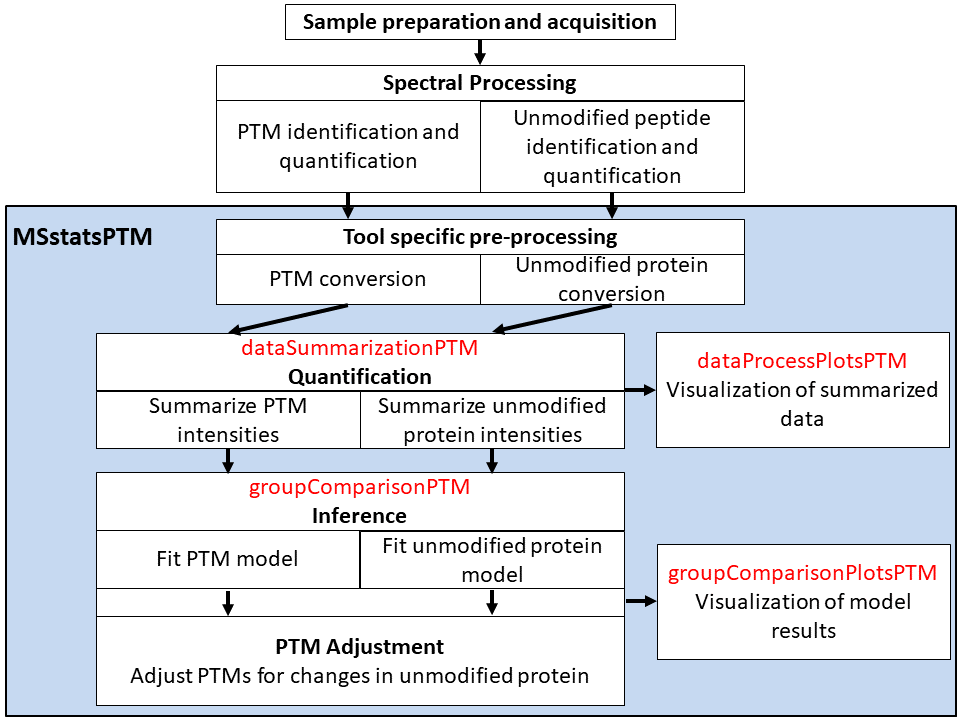
\includegraphics[scale=.8]{images/MSstatsPTM_design.png}
\caption{The workflow of MSstatsPTM and how it fits into the experimental pipeline. MSstatsPTM's workflow starts after modified and unmodified peptide quantification. First tool specific pre-processing is done, this includes modification site identification, general data cleaning, and formatting the data into the format needed for the package. The next step is feature level summarization, which summarizes features up to the modification level for the PTM data, and the protein level for the protein data. In the final step a model is fit to identify differential PTMs and unmodified proteins across conditions and the PTM model is adjusted for changes in the unmodified protein.}
\label{fig:msstatsptm_design}
\end{figure}

\begin{figure}[ht]
\centering
\begin{subfigure}[c]{0.825\linewidth}
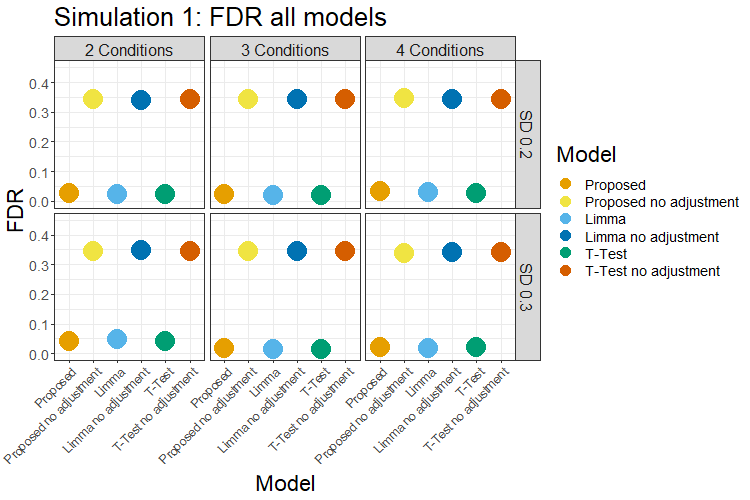
\includegraphics[width=1\textwidth]{images/sim1_FDR_all_models.png}
\caption{}
\label{fig:sim1_fdr}
\end{subfigure}
\begin{subfigure}[c]{0.825\linewidth}
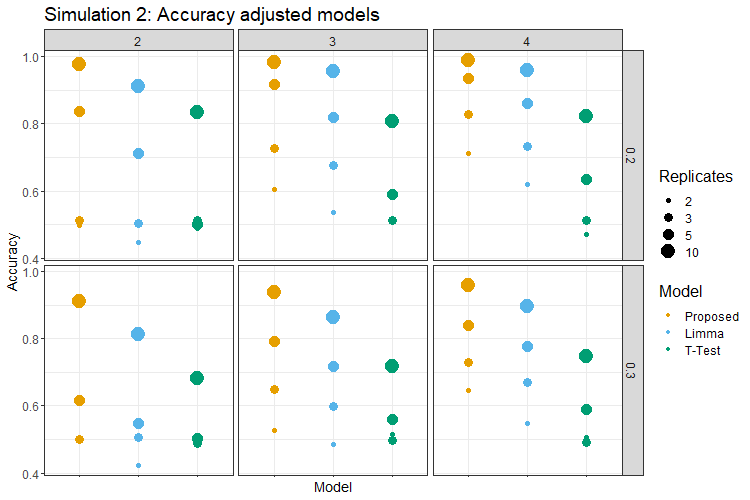
\includegraphics[width=1\textwidth]{images/sim3_Accuracy.png}
\caption{}
\label{fig:sim2_acc}
\end{subfigure}
\caption{Dataset 1 \& 2: Computer simulation. a) All the considered methods in the first computer simulation correctly calibrated FDR when adjusting for changes in protein abundance. In comparison, the methods without accounting for the protein-level changes resulted in off-target, high false positive rates. b) The advantage of using the proposed approach is apparent when including limited observations and missing values. Looking at accuracy, the proposed method outperforms Limma and t-test in nearly every model.
}
\label{fig:computer_sim}
\end{figure}


\begin{figure}[ht]
\centering
\begin{subfigure}[c]{0.825\linewidth}
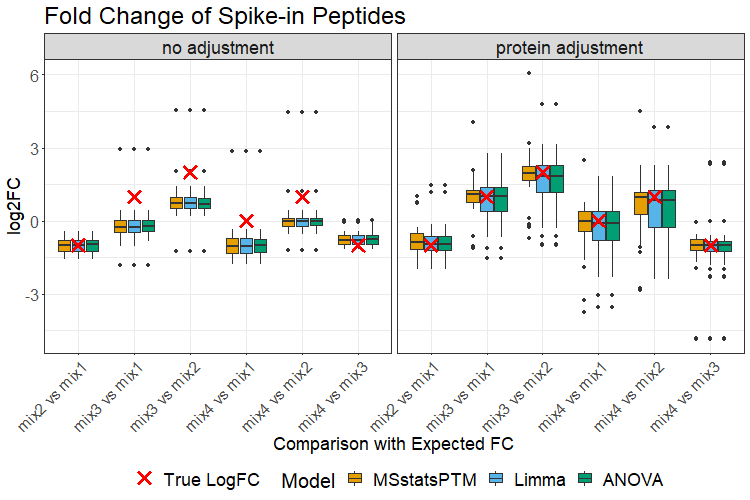
\includegraphics[width=1\textwidth]{images/spike_in_fc.png}
\caption{}
\label{fig:spikein_boxplot}
\end{subfigure}
\begin{subfigure}[c]{0.825\linewidth}
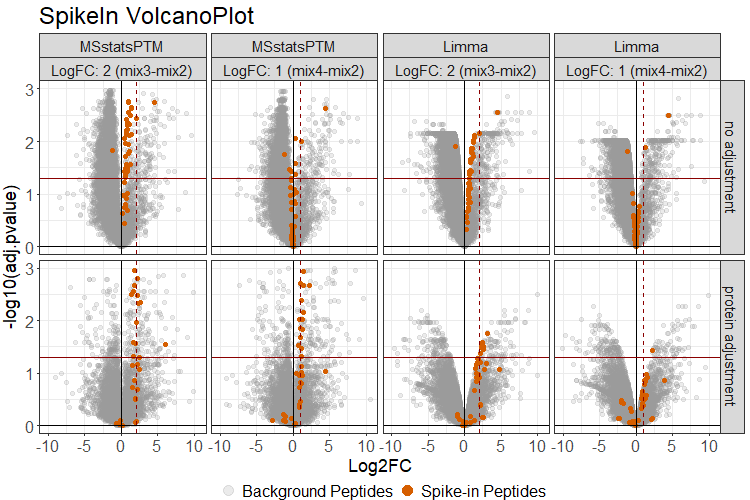
\includegraphics[width=1\textwidth]{images/spike_in_volcano.png}
\caption{}
\label{fig:spikein_prop_volcano}
\end{subfigure}
\caption{Dataset 3 : SpikeIn benchmark - Ubiquitination - Label-free. a) Before adjustment all models show the fold change of the spike-in peptides is systematically different from the expected fold change. After adjustment, this systemic difference is removed, however the inner quartile range of the Limma and t-test models is wider than the proposed method. b) The spike in peptides (colored red) do not follow the expected log fold change before adjustment. However, after adjustment, the spike in peptides are more in line with expectation. Using Limma the spike in peptides follow the expected log fold change after adjustment, however the majority of spike in peptides do not have a significant adjusted pvalue.}
\label{fig:spikein_volcano}
\end{figure}

\begin{figure}[ht]
\centering
\begin{subfigure}[c]{0.5\linewidth}
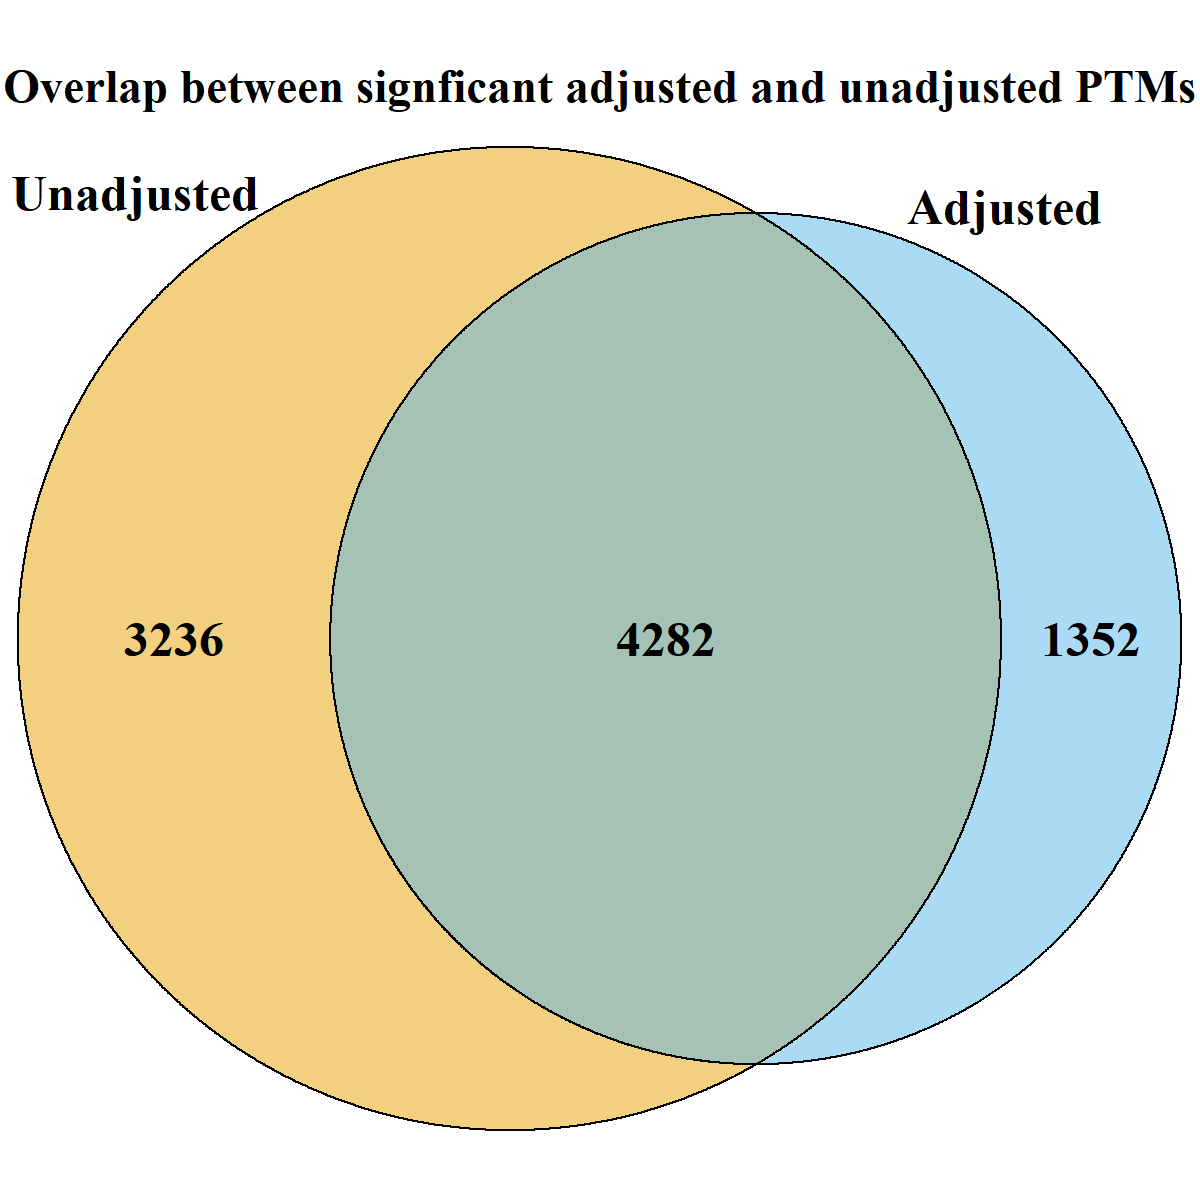
\includegraphics[width=1\textwidth]{images/ipah_venn_diagramm.png}
\caption{}
\label{fig:data4_venn_diagram}
\end{subfigure}
\begin{subfigure}[c]{0.95\linewidth}
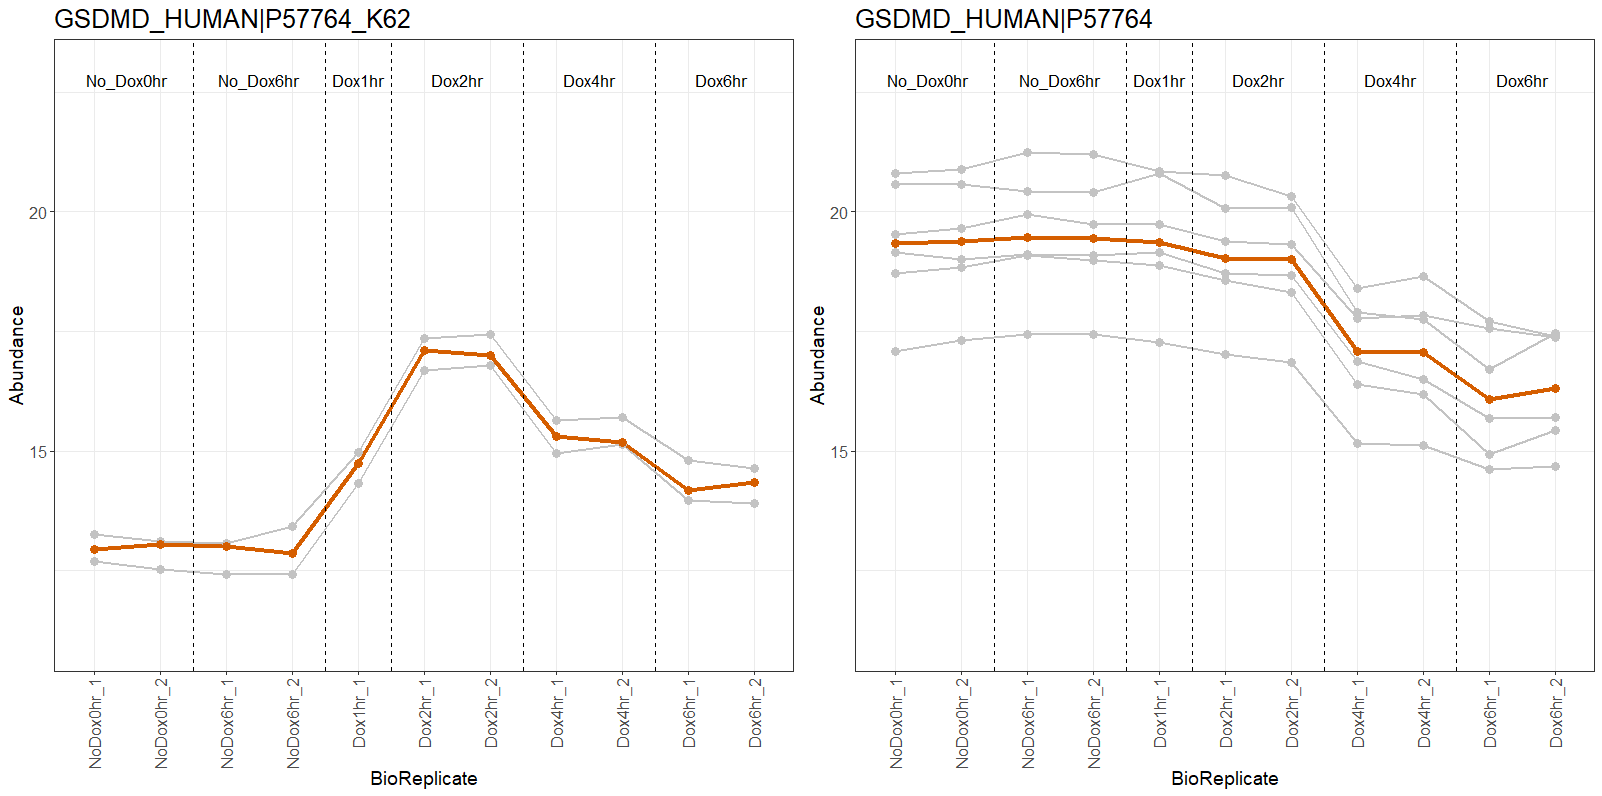
\includegraphics[width=1\textwidth]{images/IpaH_prof_plot.png}
\caption{}
\label{fig:data4_profile_plot}
\end{subfigure}
\caption{Dataset 4 : Human - Ubiquitination - 1mix-TMT. a) The overlap of differential modified peptides for the PTM model with and without global protein level adjustment. More PTMs became insignificant after adjustment then became significant. For the peptides that became insignificant in the adjusted model, their change in abundance was driven by changes in the global protein. In contrast, peptides that became significant after adjustment saw their true abundance change masked by underlying changes in the unmodified protein. b) Comparing the global profiling of protein $GSDMD$ with the ubiquitination of the protein at site $K62$. When looking at the summary of the modification and global protein it is clear the conditions follow different trends. Specifically, there appears to be no change in abundance between Dox1hr and Dox4hr in the modified plot, however there is a large negative change when looking at the unmodified plot. This indicates the modification is confounded with changes in the unmodified protein.}
\label{fig:data4_plots}
\end{figure}

\begin{figure}[h!]
\centering
\begin{subfigure}{\textwidth}
 \centering
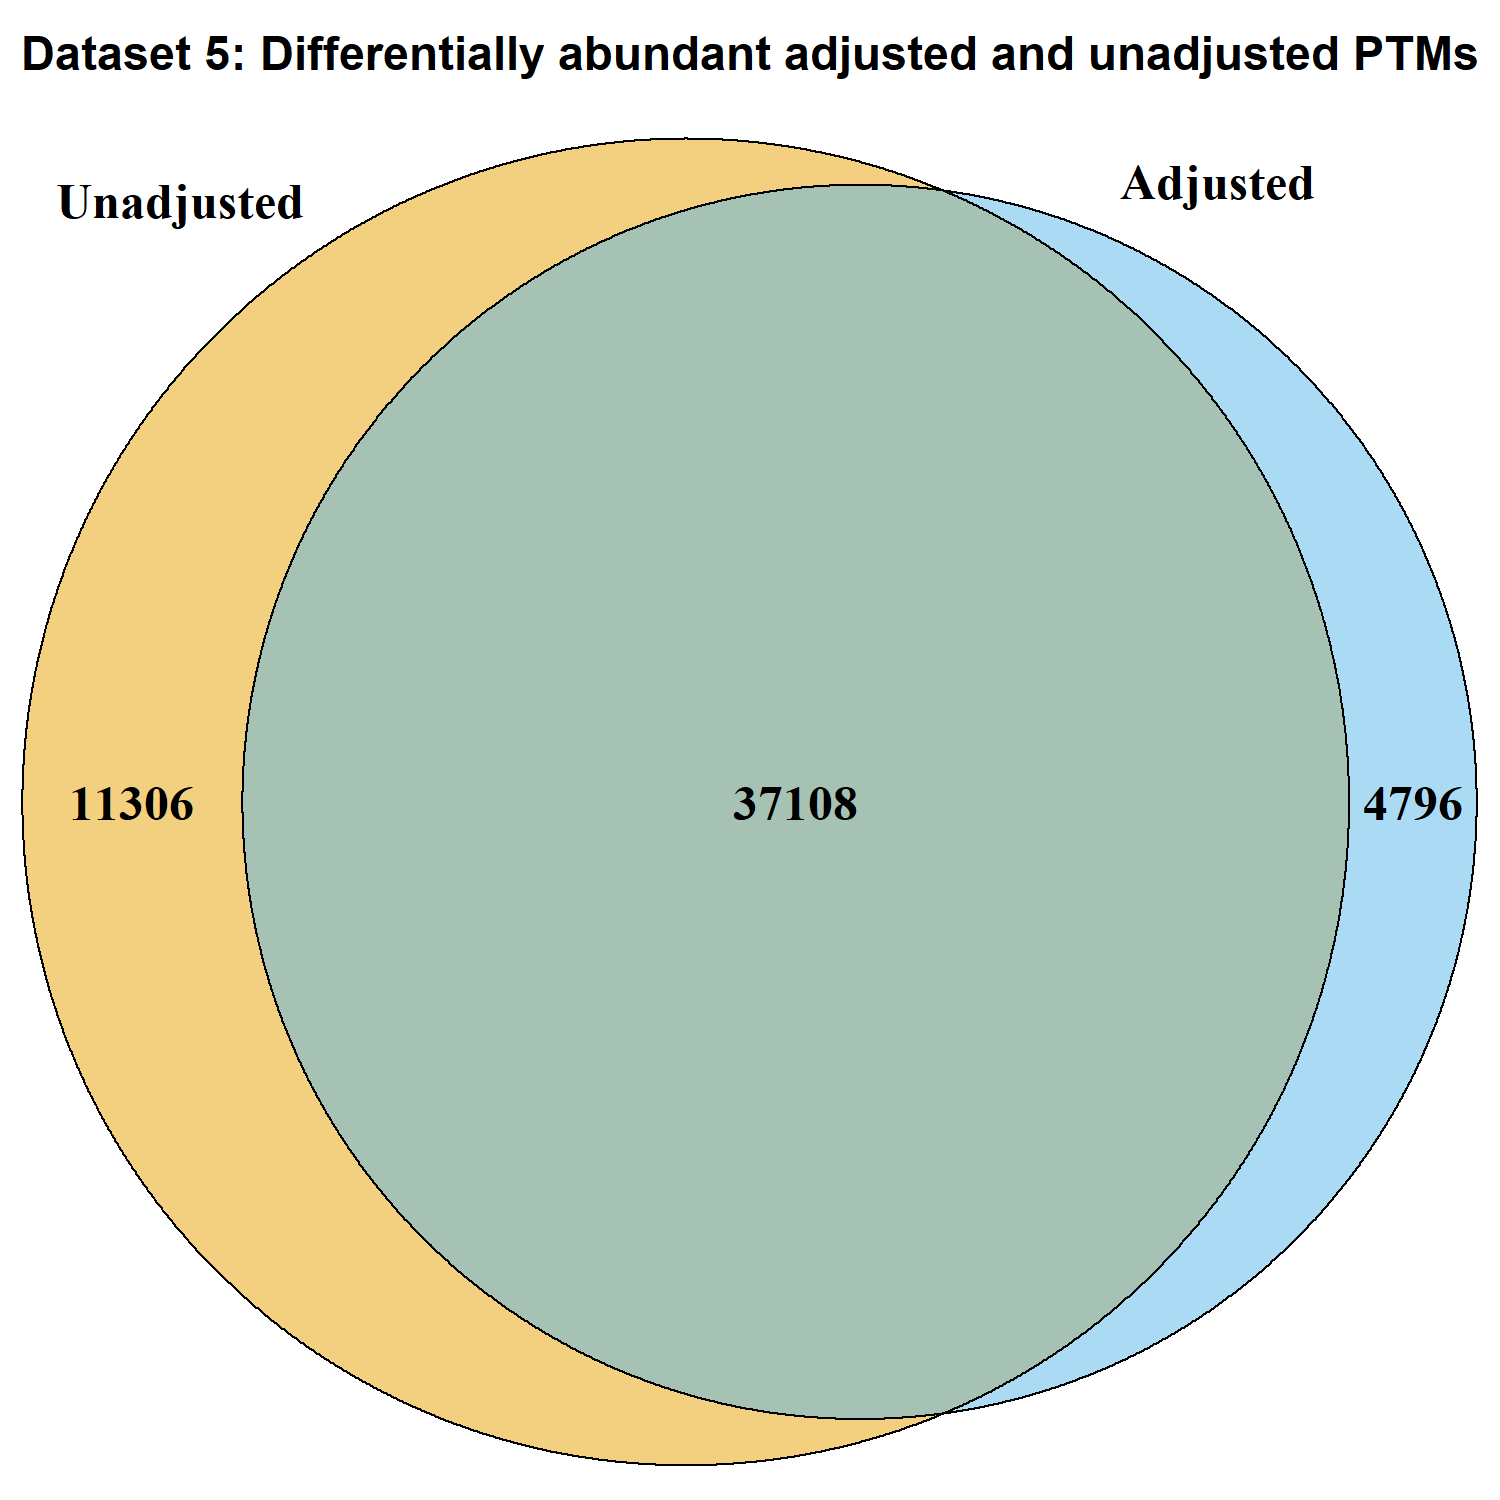
\includegraphics[height=.5\textwidth]{images/shig_venn_diagramm.png}
\caption{}
\label{fig:data5_venn_diagram}
 \end{subfigure}
 \begin{subfigure}{\textwidth}
 \centering
	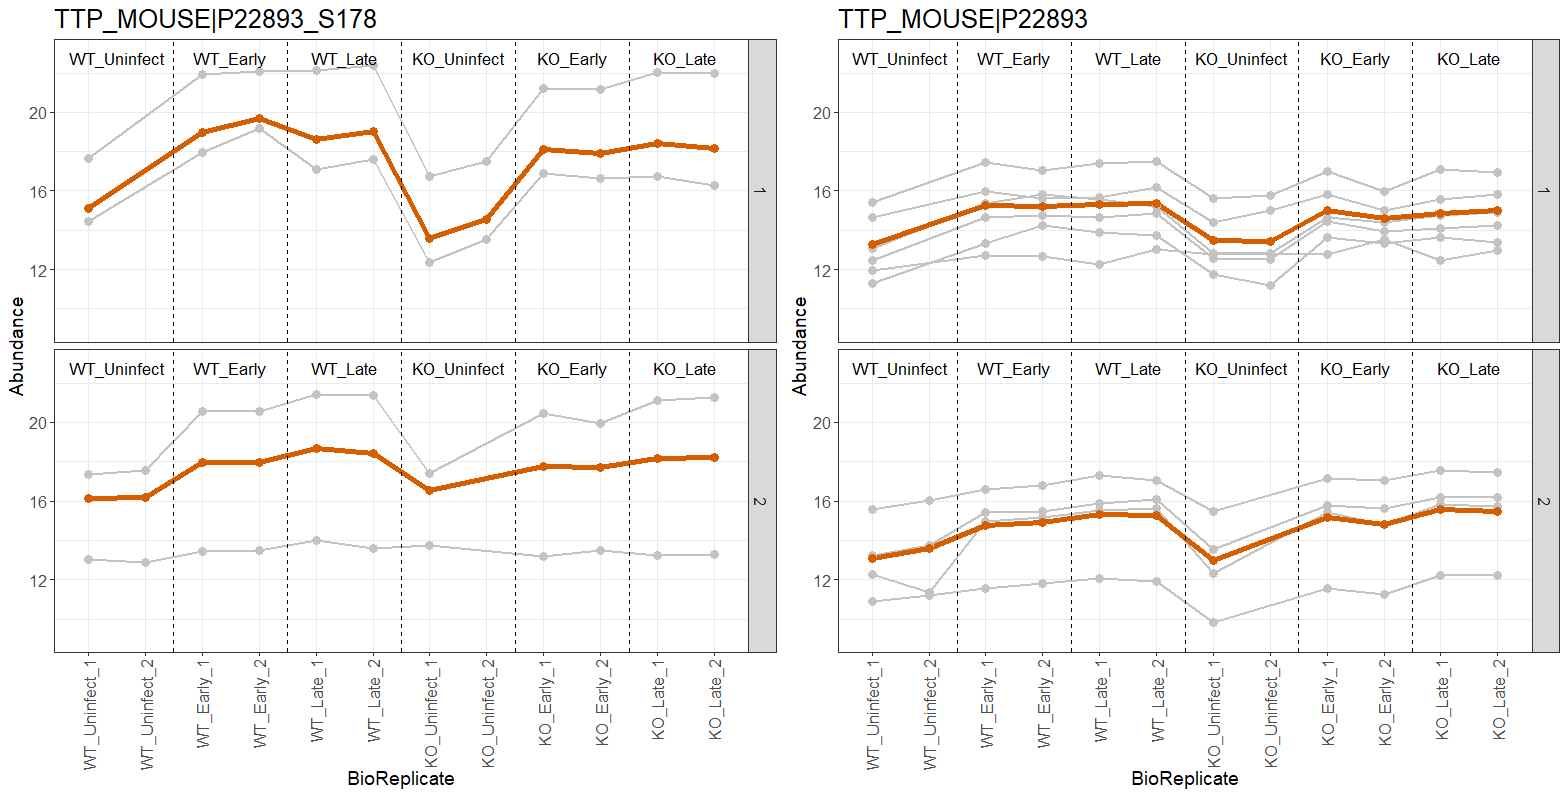
\includegraphics[width=1.0\textwidth]{images/No_Difference_Shigella_Profile_Plot}
	\caption{}
	\label{fig:data5_profile_plot}
	 \end{subfigure}
\caption{Dataset 5 : Mouse - Phosphorylation - 2mix-TMT time series. a) The overlap of differentially modified peptides between the PTM model with and without global protein level adjustment. Again more PTMs became insignificant after adjustment then became significant. Comparing the global profiling of protein $TTP$ with the modification of the protein at site $S178$. When looking at the summary of the modification and global protein it is clear the difference between conditions follow the same trend. Specifically, there is a positive adjustment in abundance when comparing WT\_Uninfect to WT\_Late in both the modification and global profiling run. This indicates the movement is driven by changes in global protein that is only accounted for in the model when adjusting for global protein abundance change.}
\label{fig:data5_plots}
\end{figure}

\begin{figure}[h!]
\centering
 \begin{subfigure}{\textwidth}
 \centering
	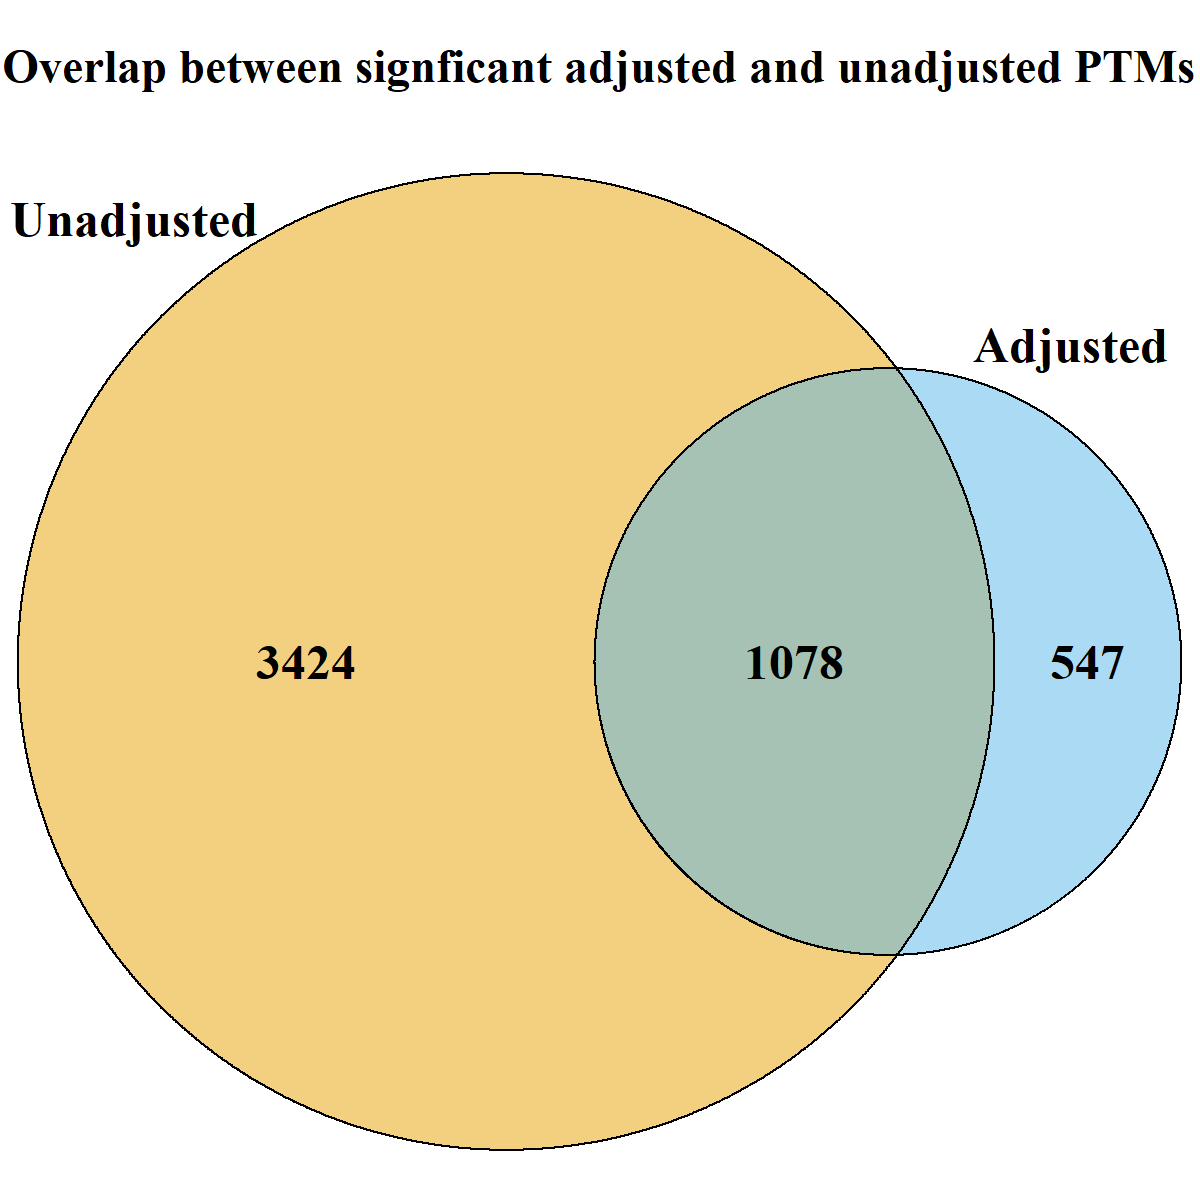
\includegraphics[height=.525\textwidth]{images/usp30_venn_diagramm}
	\caption{}
	\label{fig:data6_vd1}
 \end{subfigure}
 \begin{subfigure}{\textwidth}
 \centering
	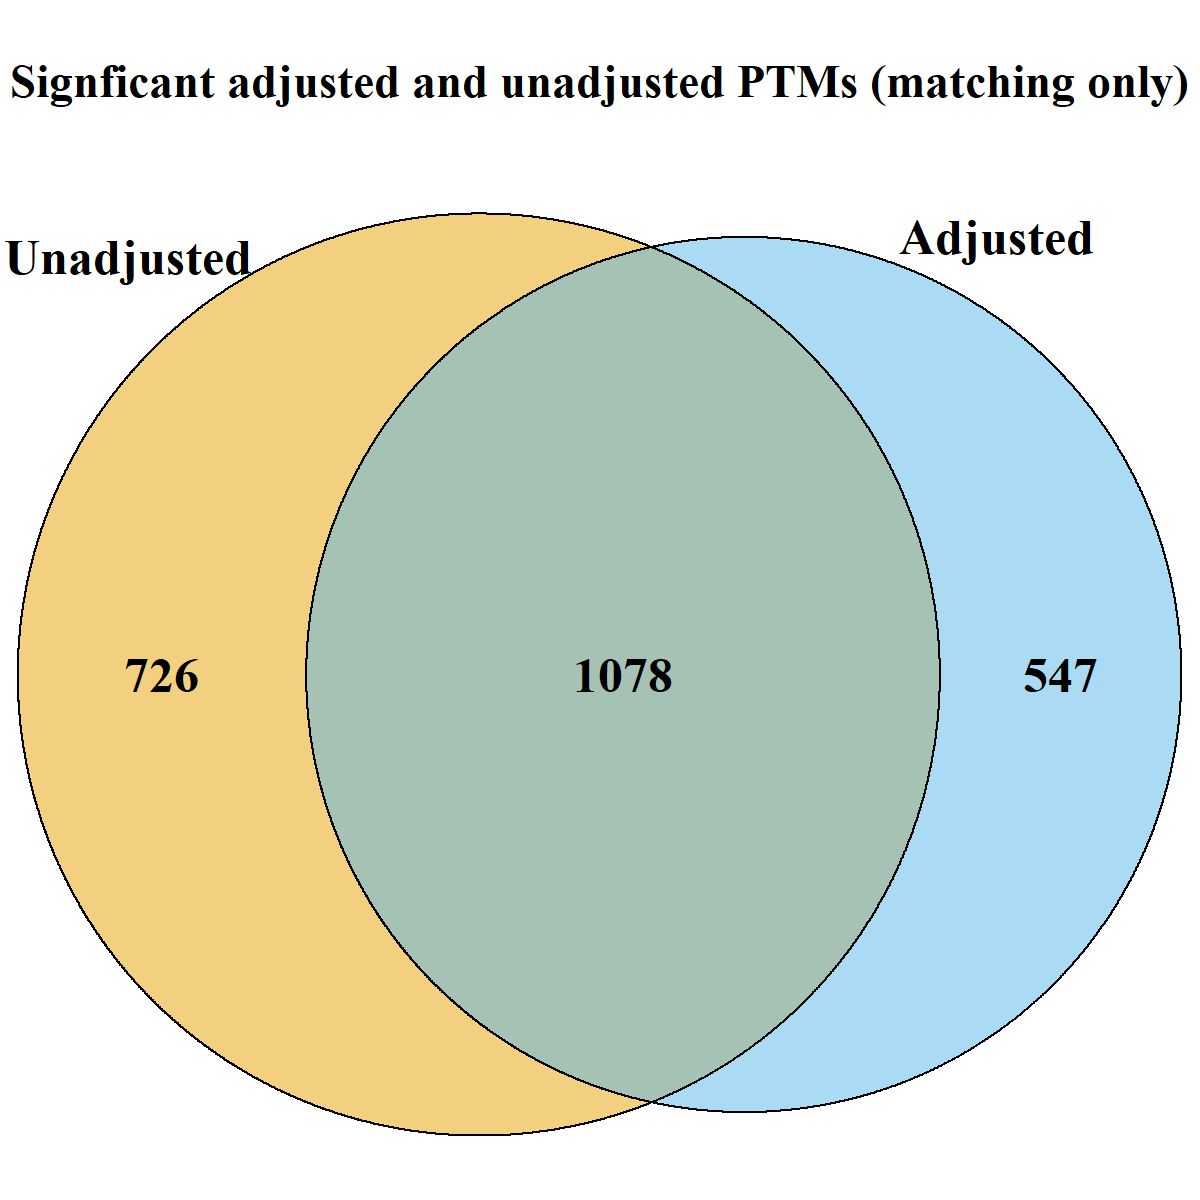
\includegraphics[height=.525\textwidth]{images/usp30_venn_diagramm_matching_only}
	\caption{}
	\label{fig:data6_vd2}
 \end{subfigure}
 \caption{Dataset 6 : Human - Ubiquitination - Label-free no global profiling run. a) The overlap of differencial modified peptides for the PTM model with and without global protein level adjustment. Here many more PTMs became insignificant then became significant after adjustment. This is due to not having a global profiling run, resulting in a large lack of overlap between the modified peptides and unmodified proteins. b) Here we make the same comparison but only for modified peptides with a matching unmodified protein, so adjustment can be performed. In this case we see significantly less peptides become insignificant after adjustment. This highlights the need for a global profiling run if protein adjustment is going to performed.}
\label{fig:data6_plots}
\end{figure}

%\begin{figure}[h!]
%\centering
% \begin{subfigure}{\textwidth}
% \centering
%	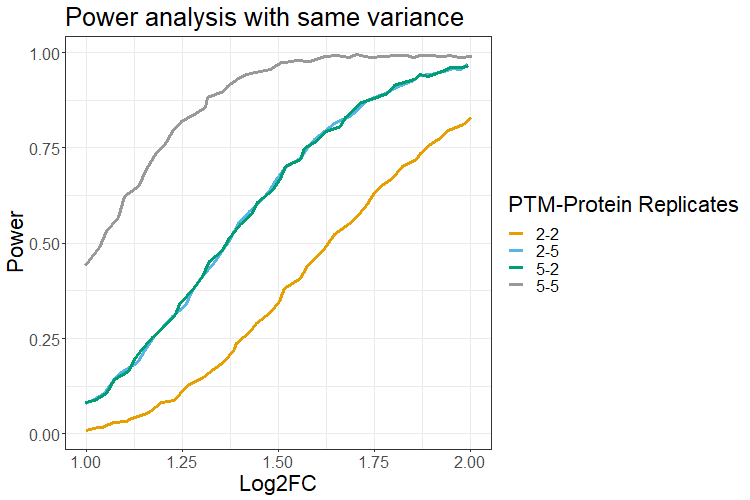
\includegraphics[width=.75\textwidth]{images/same_var_power}
%	\caption{}
% \end{subfigure}\vspace{5mm}
% \begin{subfigure}{\textwidth}
% \centering
%	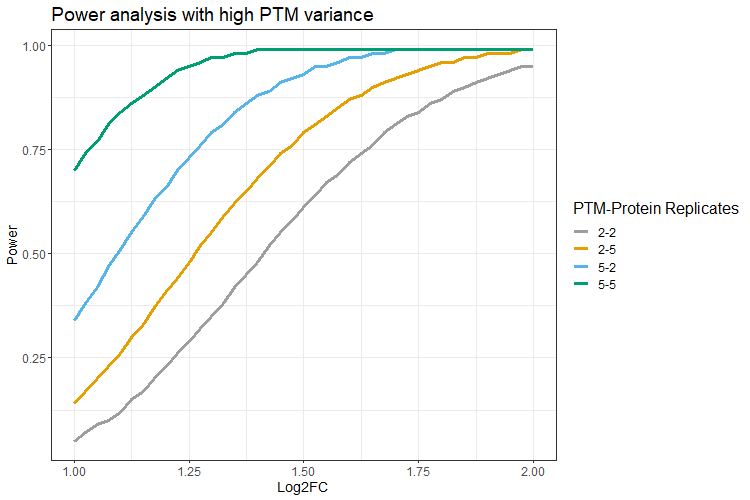
\includegraphics[width=.75\textwidth]{images/high_ptm_var_power}
%	\caption{}
% \end{subfigure}
% \caption{Power analysis of experiments with differing variances. a) The power of an experiment targeting PTMs with the same variance, .15, for the modified and unmodified peptides. Predictably when the replicates are high for both modified and unmodified peptides the power is much higher. Conversely at low replicates for each the power is much lower. The interesting part of this chart is when the replicates are different between runs. With equal variance, it does not matter if the PTM replicates or protein replicates are higher. b) In this chart the variance for the PTM is higher than the unmodified protein. The PTM variance is .2, while the unmodified protein variance is .1. With equal replicates the results are the same as above, more replicates equals more power. When the replicates are not the same we can clearly see that having more replicates for the PTM leads to higher power.}
%\label{fig:power_sd_combo}
%\end{figure}


\end{document}
